\documentclass[conference]{IEEEtran}
\IEEEoverridecommandlockouts
% The preceding line is only needed to identify funding in the first footnote. If that is unneeded, please comment it out.
\usepackage[style=numeric]{biblatex}
\addbibresource{citations.bib}
\usepackage{amsmath,amssymb,amsfonts}
\usepackage{minted}
\usepackage{algorithmic}
\usepackage{graphicx}
\usepackage{listings}

\usepackage{textcomp}
\usepackage{xcolor}
\def\BibTeX{{\rm B\kern-.05em{\sc i\kern-.025em b}\kern-.08em
    T\kern-.1667em\lower.7ex\hbox{E}\kern-.125emX}}
\begin{document}

\title{Smart Parking Lot Assist System\\
{\footnotesize \textbf{
    Final Report \\
    Submitted in partial fullfilment of the requirements for senior design project\\
    Electrical and Computer Engineering Department \\
    Rutgers University, Piscataway, NJ 08854 \\
}
}
}

\author{
\textbf{Rajeev Atla, Parshva Mehta, Aman Patel, Abhiram Vemuri} \\
Advisor: Kristin Dana\\
Team Number: SP25-02 
}

\maketitle

\begin{abstract}
    As transport infrastructure grows increasingly complex, 
    large universities face increasing challenges in meeting the parking demands of students and faculty, 
    especially with continued reliance on personal vehicles. 
    Previous attempts to improve parking through automated valet systems have failed mainly due to high costs and logistical difficulties. 
    In campus environments, 
    shifting schedules and limited staff availability further complicate these solutions, 
    resulting in drivers often wasting time circling crowded lots, 
    causing congestion and increased emissions.
    This project introduces a scalable Smart Parking Assist System to address these issues that leverages computer vision and a web application to provide real-time parking detection and guidance. 
    The system comprises three core components: 
    the Machine Learning Model, 
    the Hardware Setup, 
    and the User Application.
    The machine learning component begins with dataset collection, 
    combining public datasets with images from the CoRE building. 
    These are preprocessed and then used to train a YOLO-based model capable of accurately classifying parking spaces. 
    The trained model weights are deployed to the hardware module.
    The hardware consists of a Raspberry Pi and a high-resolution camera capturing parking lot images and performing on-device inference. 
    Outputs are formatted as JSON and sent to the backend.
    The application includes both a frontend and a backend. 
    The backend converts JSON data to CSV, 
    updates a central database, 
    and connects to the frontend. 
    The frontend delivers real-time updates, 
    allowing users to locate available spaces efficiently.
    These components create a seamless, 
    scalable, 
    real-time parking solution suitable for university campuses and urban environments.    
\end{abstract}

\begin{IEEEkeywords}
    Computer Vision, Full-stack Development, Machine Learning, Data Pipelining/Manipulation
\end{IEEEkeywords}

\section{Introduction}
As transport infrastructure grows increasingly complex, 
large universities face mounting challenges in meeting the parking needs of students and faculty, 
especially with the continued reliance on individual car commuting. 
This project proposes an integrated solution using security camera imaging, 
computer vision, 
and a simple mobile application to ease the process of finding parking. 
The solution consists of two key components. 
First, 
a custom-configured security camera will be installed to overlook campus parking lots,
capturing high-resolution images. 
These images are processed through a computer vision model, 
pre-trained to detect open parking spaces with high accuracy. 
The output from this model is then converted into a dynamic dataset identifying available parking spots in real-time. 
Second, 
this dataset is seamlessly integrated into a user-friendly mobile application focused on clarity and ease of use. 
The app features an adaptive interface with real-time maps, 
filters, 
and notifications, 
enabling users to quickly locate free parking spaces near their destinations and make more informed parking decisions. 
Past attempts to improve parking with automated valet systems have failed, 
often because of high costs, 
complicated logistics, 
and issues with reliability. 
In a lively campus setting, 
these valet systems could be more feasible: 
changing class schedules, 
various modes of transportation, 
and limited staff availability make it hard to provide reliable valet services. 
As a result, 
drivers waste precious time driving in circles in busy lots, 
leading to congestion, 
frustration, 
and adverse environmental effects. 
By combining advanced imaging technology with intuitive design, 
this project aims to enhance the daily commuting experience for students and faculty. 
Moreover, 
integrating this information into an accessible platform contributes to the broader goal of fostering sustainable and efficient urban mobility patterns, 
paving the way for data-driven transportation solutions on and beyond university campuses.

\section{Approach Methods}

\subsection{Dataset Prep}

The foundation of this project is a diverse and robust dataset comprising parking lot images with varying occupancy levels \cite{dataset_images}, 
\cite{images_original}. 
The dataset includes images collected from both public sources and proprietary captures using our camera system, 
ensuring strong relevance to real-world conditions. 
During preprocessing, 
resizing, 
normalization, 
and data augmentation techniques are applied to improve data quality and simulate various environmental scenarios such as lighting changes and occlusions. 
Each image is carefully annotated to label parking spaces as occupied or vacant. 
Special categories such as handicapped spots, 
electric vehicle charging stations,
and reserved parking spaces receive particular attention to enhance the system’s practical utility. 
These steps result in a high-quality, 
well-labeled dataset that supports effective model training and contributes significantly to the system’s accuracy and reliability.

\subsection{ML Model}



This project leverages the YOLOv11 (You Only Look Once) 
computer vision algorithm \cite{yolo11_ultralytics} 
to address the task of parking space detection. 
Known for its speed and accuracy, 
YOLOv11 is well-suited for real-time applications, 
especially on resource-constrained platforms. 
The model undergoes customization and fine-tuning to tackle the specific challenges of parking detection, 
including variations in vehicle size, 
overlapping boundaries, 
and partial occlusions from objects or shadows. 
Advanced image processing techniques are integrated to maintain detection reliability under diverse weather conditions and inconsistent image quality. 
Training focuses on maximizing accuracy while reducing computational load to enable smooth operation on low-power devices like the Raspberry Pi. 
Techniques such as quantization and pruning help reduce model complexity without sacrificing performance. 
Rigorous testing and validation ensure the model performs robustly across a range of environments. 
The annotated datasets developed earlier in the project are used to evaluate and refine the model, 
improving its real-time accuracy and effectiveness.

\subsection{Hardware}

Selecting the Raspberry Pi 5 and a compatible camera module plays a key role in the success of this project. The Raspberry Pi 5 provides the necessary processing power and connectivity to support smooth, stable operation of the machine learning model without outages or connection issues. A secure mounting system ensures the camera remains in a fixed position, producing consistent image captures critical for accurate detection. The testing phase evaluates the system’s hardware stability, image quality, and model performance across a variety of parking lot layouts. Extensive field testing helps fine-tune the integration and optimize the system for real-world deployment. In cases where the Raspberry Pi 5 cannot handle full model inference locally due to computational limits, the system is configured to offload processing to an external computer. In such setups, the Raspberry Pi 5 transmits images over Wi-Fi or Ethernet, maintaining its role as the edge capture and communication device.

\subsection{Software}
The software component of the system integrates advanced image processing, machine learning, and user-facing features to deliver a complete parking detection solution. Captured images are first processed through steps such as noise reduction, color correction, and enhancement to ensure high-quality inputs for the trained model. The inference pipeline uses the YOLOv11 model to detect and classify parking spaces in real time with high accuracy and low latency. Data transmission is handled through reliable communication protocols such as Wi-Fi or cellular networks, enabling seamless integration with either a central server or a mobile application.

The web application functions as the primary interface for users, displaying real-time parking availability through interactive maps, search tools, and live notifications. Available parking spots are clearly highlighted, helping users quickly identify open spaces in specific lots. The processed outputs from the machine learning model are sent to the app’s backend, which then updates the front-end user interface with up-to-date parking status. Special attention is given to creating an intuitive and responsive design that works across a range of devices and user preferences, ensuring the system is accessible and practical for everyday use.


\section{Challenges}
Throughout the development of our project, 
we encountered several significant challenges related to regulation and the supply chain, 
which ultimately limited the performance and scope of our system. 
Initially, 
the project was designed to utilize an aerial camera perspective, 
similar to the dataset images 
(see Figure \ref{fig:fig4}), 
in order to accurately capture parking lines and define bounding boxes around each space. 
However, 
due to regulatory constraints from Rutgers University and the State of New Jersey, 
we were not permitted to install cameras on elevated platforms or drones as originally planned. 
As a result, 
we had to revise our approach and instead placed a stationary camera on the 5th floor of the CoRE building. 
This new vantage point introduced several visibility issues, 
as many parking spots were blocked by vehicles already parked in front of them, 
reducing the clarity and reliability of our input images. 

In addition to these regulatory limitations, 
we also faced delays in receiving essential hardware components. 
The camera's power supply and SD card arrived late in the semester, 
preventing us from fully setting up and testing the system on-site. 
This significantly limited our ability to collect real-world data from the intended parking lot, 
which in turn negatively impacted the accuracy and effectiveness of our trained model. 
The power supply and SD card arriving late has significantly impacted the ability to continue building the system pipeline. 
The goal was to have the camera take a continuous video, 
house the YOLOv11 model on the Raspberry Pi itself for local computing, 
take images at regular intervals with bounding boxers overlayed, 
send images to a database, 
pull the information from these images, 
and update a website with this information. 
Our development timeline has been dramatically affected by these issues.

Particularly on the software end of the project, 
the delay in receiving the hardware components needed to execute our project has drastically changed the way our database is being updated. 
The output of our ML model program needs to be used to update the database, 
but due to not having access to the power supply and SD card to fully test the system, 
we had to develop a workaround method for simply getting real data from the parking lot. 
The workaround we resorted to was using our phone cameras, 
which resulted in some limitations compared to what was originally envisioned such as lower quality resolution, 
and inconsistent frame rates of mobile devices. 
This made it harder for the ML algorithm to detect vacant or occupied parking spaces, 
which can result in missed or incorrect detections affecting the output file of the ML algorithm after running it and using the updated CSV file to update the database. 
These inaccuracies propagated through the pipeline resulting in a few false positives, 
resulting in a few incorrect entries into the database. 

Another problem that was encountered was when trying to optimize the refresh rate for database stability and accuracy. 
Initially our system was trying to update the database every 5 to 10 seconds from reading the CSV file, 
but this had several implications such as the database locking, 
writing conflicts, 
and also occasional crashes when running the server for frontend requests. 
In order to solve this the refresh interval was increased to 30 seconds to avoid instability in the database system. 
This eased the load on the database, 
kept the access conflicts with the frontend requests to a minimal amount, 
and allowed the ML model more time to process images and get higher quality outputs closer to the real-time scenario. 
Overall, 
this more refined approach allowed for a more sustainable balance between the backend functionality of the system and the real-time data generated by the ML model.

\section{Results}

During the model training phase, 
a fine-tuning strategy was employed due to the absence of prior knowledge regarding the optimal number of training epochs. 
This approach involved training the model for a fixed number of epochs to obtain an initial set of weights. 
These weights were then used to initialize the model for subsequent training cycles, 
effectively serving as a foundation for further refinement. 
This iterative weight generation and retraining process was repeated across multiple rounds, 
allowing for gradual performance improvements while mitigating the risk of overfitting or underfitting.

We begin by analyzing the training and validation loss curves to evaluate the learning behavior of the model throughout the training process. 
These plots provide insight into the model’s convergence and potential overfitting or underfitting tendencies.

\subsection{Training Loss}

Figure \ref{fig:fig1} illustrates the progression of the training loss throughout the training process. 
During the early epochs,
the training loss exhibits fluctuations as the optimizer begins to interact with the training data. 
These fluctuations indicate the optimization process adjusting to the model’s parameters and gradually improving the model's ability to minimize the loss. 
In the subsequent epochs,
the loss shows a steady decrease, 
demonstrating that the model is learning from the data and the optimizer is refining its parameters effectively.

The large fluctuations occur near the start of training, 
indicating a high learning rate near the start. 
The loss decreases drastically during this time. 
As the training progresses, 
the loss curve begins to plateau after around 750-800 epochs, 
with the loss stabilizing at approximately 0.6. 
This plateau indicates that the model is nearing convergence, 
meaning that the learning process is reaching a point where improvements are marginal, 
and the model's parameters have largely stabilized. 
The slight oscillations in the plot, 
particularly the ''spikes,'' 
correspond to moments of fine-tuning, 
where the optimizer undergoes specific adjustments to the model's weights. 
These fluctuations are expected, 
as fine-tuning allows for more nuanced adjustments, 
enhancing the model’s performance while avoiding drastic shifts in the learned parameters.

The consistent rise and fall of the loss during these fine-tuning periods reflects the adaptive nature of the training process. 
Notably, 
each fine-tuning cycle results in the loss ultimately decreasing to a lower value than the previous cycle, 
demonstrating effective model refinement. 
The general trend of the training loss decreasing over time and ultimately plateauing reinforces the model's capacity to converge toward an optimal solution.

\begin{figure}[h]
    \centering
    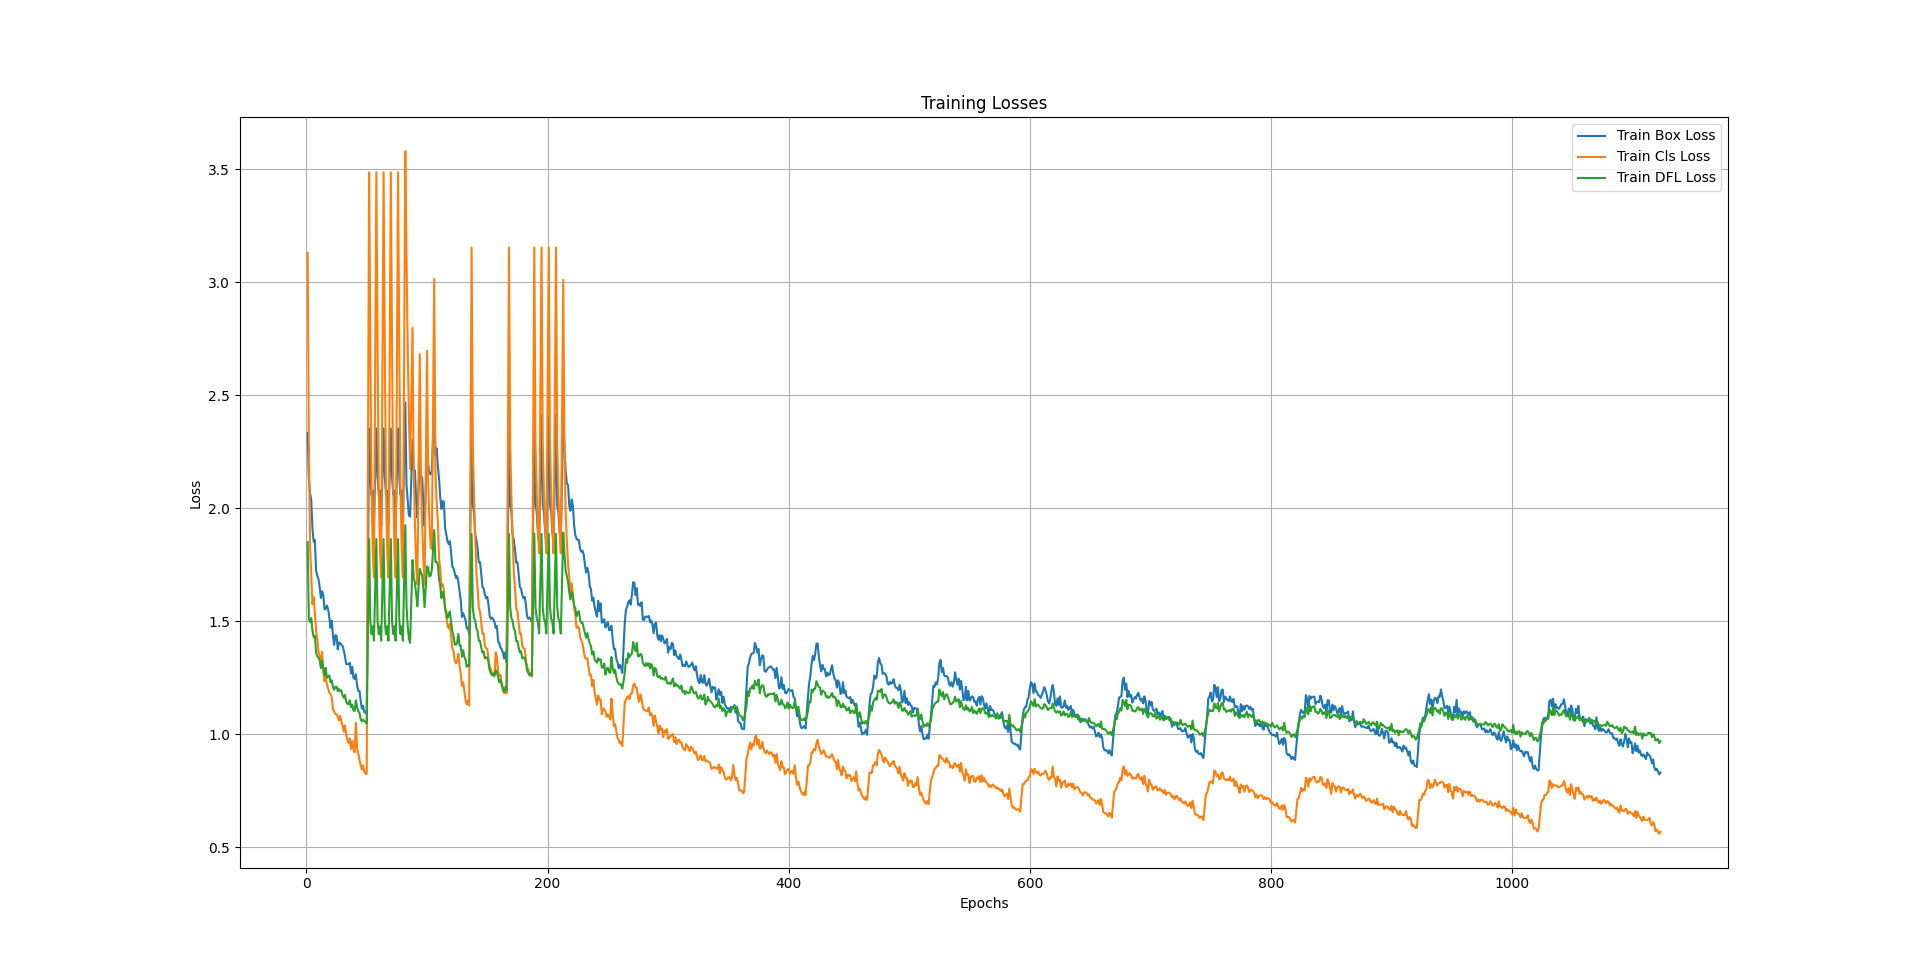
\includegraphics[scale=0.2]{Figure_1.png}
    \caption{
        Notice how the training loss generally decreases throughout the training and plateaus after 750-800 epochs at a value of 0.6. 
        The ''spikes'' in the beginning and throughout the plot represent fine-tuning.
    }
    \label{fig:fig1}
\end{figure}

\subsection{Validation Loss}

Figure \ref{fig:fig2} shows the progression of the validation loss throughout the training process. 
Initially, 
the validation loss decreases steadily, 
mirroring the trend observed in the training loss. 
However, 
as training continues, 
the rate of improvement slows, 
and the loss begins to plateau around 750-800 epochs. 
This plateau suggests that the model is reaching a point of diminishing returns, 
where further training would yield only marginal improvements in validation performance. 
The model’s ability to generalize to unseen data stabilizes, 
indicating that it has learned the underlying patterns effectively without overfitting.

The presence of spikes in the validation loss plot is similar to those in the training loss. 
These fluctuations correspond to periods of fine-tuning, 
where the optimizer makes targeted adjustments to the model’s weights. 
Fine-tuning helps refine the model's performance, 
ensuring it is better equipped to generalize to unseen data. 
These minor increases in validation loss reflect the optimizer's effort to fine-tune the learned parameters, 
balancing between exploration and exploitation of the parameter space. 
While these fluctuations are visible, 
they do not significantly detract from the overall downward trend of the validation loss.

The plateau observed after 750-800 epochs indicates that the model has achieved stability in its learning. 
At this stage, 
continuing training would likely lead to overfitting, 
where the model’s performance on the validation set would begin to degrade. 
Therefore, 
the training was halted at this point to avoid overfitting and ensure that the model maintained its generalization capability. 
The validation loss plot highlights the effectiveness of this strategy, 
demonstrating that the model achieved its optimal performance without unnecessary overtraining.



\begin{figure}[h]
    \centering
    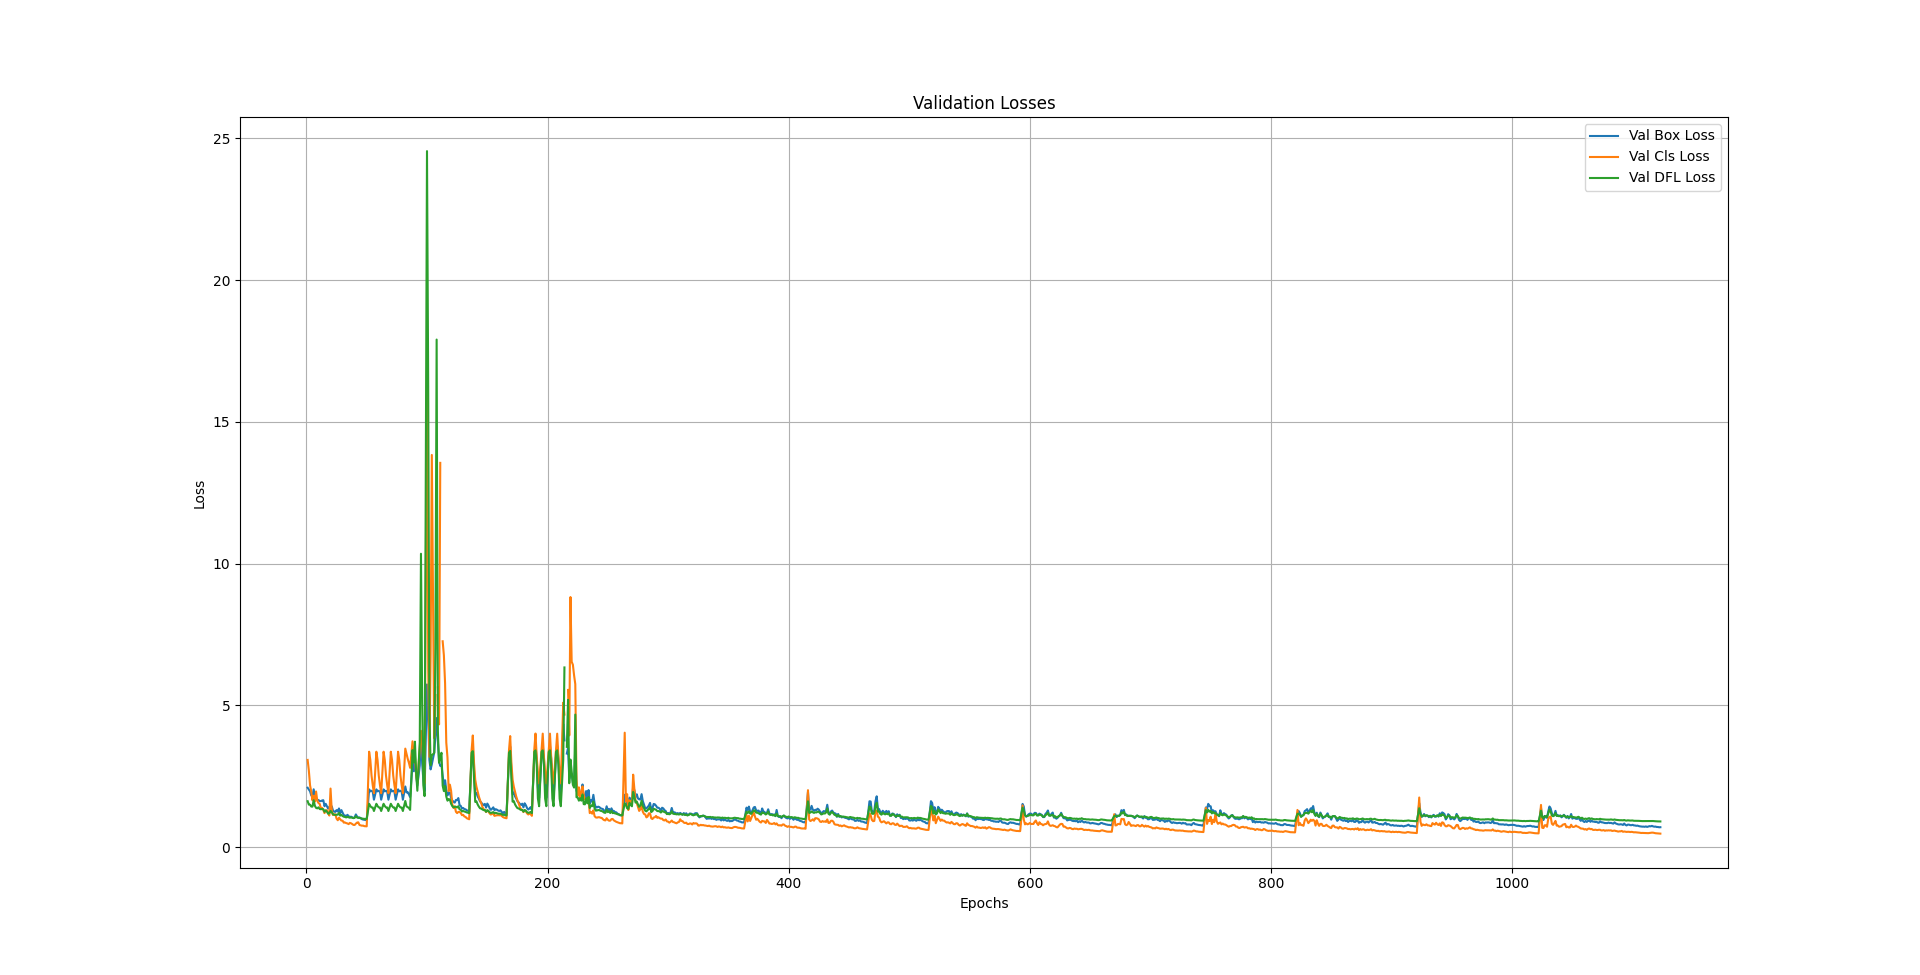
\includegraphics[scale=0.2]{Figure_2.png}
    \caption{
        Notice how the validation loss generally decreases and plateaus after 750-800 epochs. 
        When training the model, 
        the stopping point was when the validation loss plateaus. 
        The spikes are present in this plot as well.    
    }
    \label{fig:fig2}
\end{figure}

\subsection{Evaluation}

Figure \ref{fig:fig3} presents the evolution of the four evaluation metrics: 
Precision (P), 
Recall (R), 
mAP50 (Mean Average Precision), 
and mAP50-95. 
As shown, 
the values of all four metrics consistently increase over the course of training, 
indicating improvements in the model’s performance as it learns from more data. 
Precision steadily rises, 
reaching a final value of approximately 0.87, 
reflecting the model's growing accuracy in detecting objects. 
Recall increases as well, 
reaching around 0.80, 
suggesting that the model is becoming better at identifying all instances of objects in the images. 
Both mean average precision (mAP)
metrics demonstrate a similar upward trend, 
with mAP50 finishing at about 0.90 and mAP50-95 concluding at 0.72. 
These scores indicate improvements in the model's accuracy across different levels of detection difficulty and at various IoU thresholds \cite{yolo11_ultralytics}.

The occasional spikes in the evaluation metrics are consistent with the fine-tuning process, 
as observed in the training and validation loss plots. 
These fluctuations represent moments when the optimizer adjusts the model’s weights, 
leading to short-term increases in performance before stabilizing again. 
Despite these minor oscillations, 
the overall trajectory of the metrics is clear: 
the model becomes more accurate and better able to generalize over time, 
as evidenced by the steady improvement across all four metrics.

These results are crucial for evaluating the model’s ability to perform object detection effectively. 
The improvements in precision and recall suggest that the model is not only becoming more accurate in its detections but is also identifying a larger proportion of the objects in the images. 
The increasing mAP scores further reinforce this, 
indicating that the model is refining its detection capabilities and performing well across various detection scenarios.

\begin{figure}[h]
    \centering
    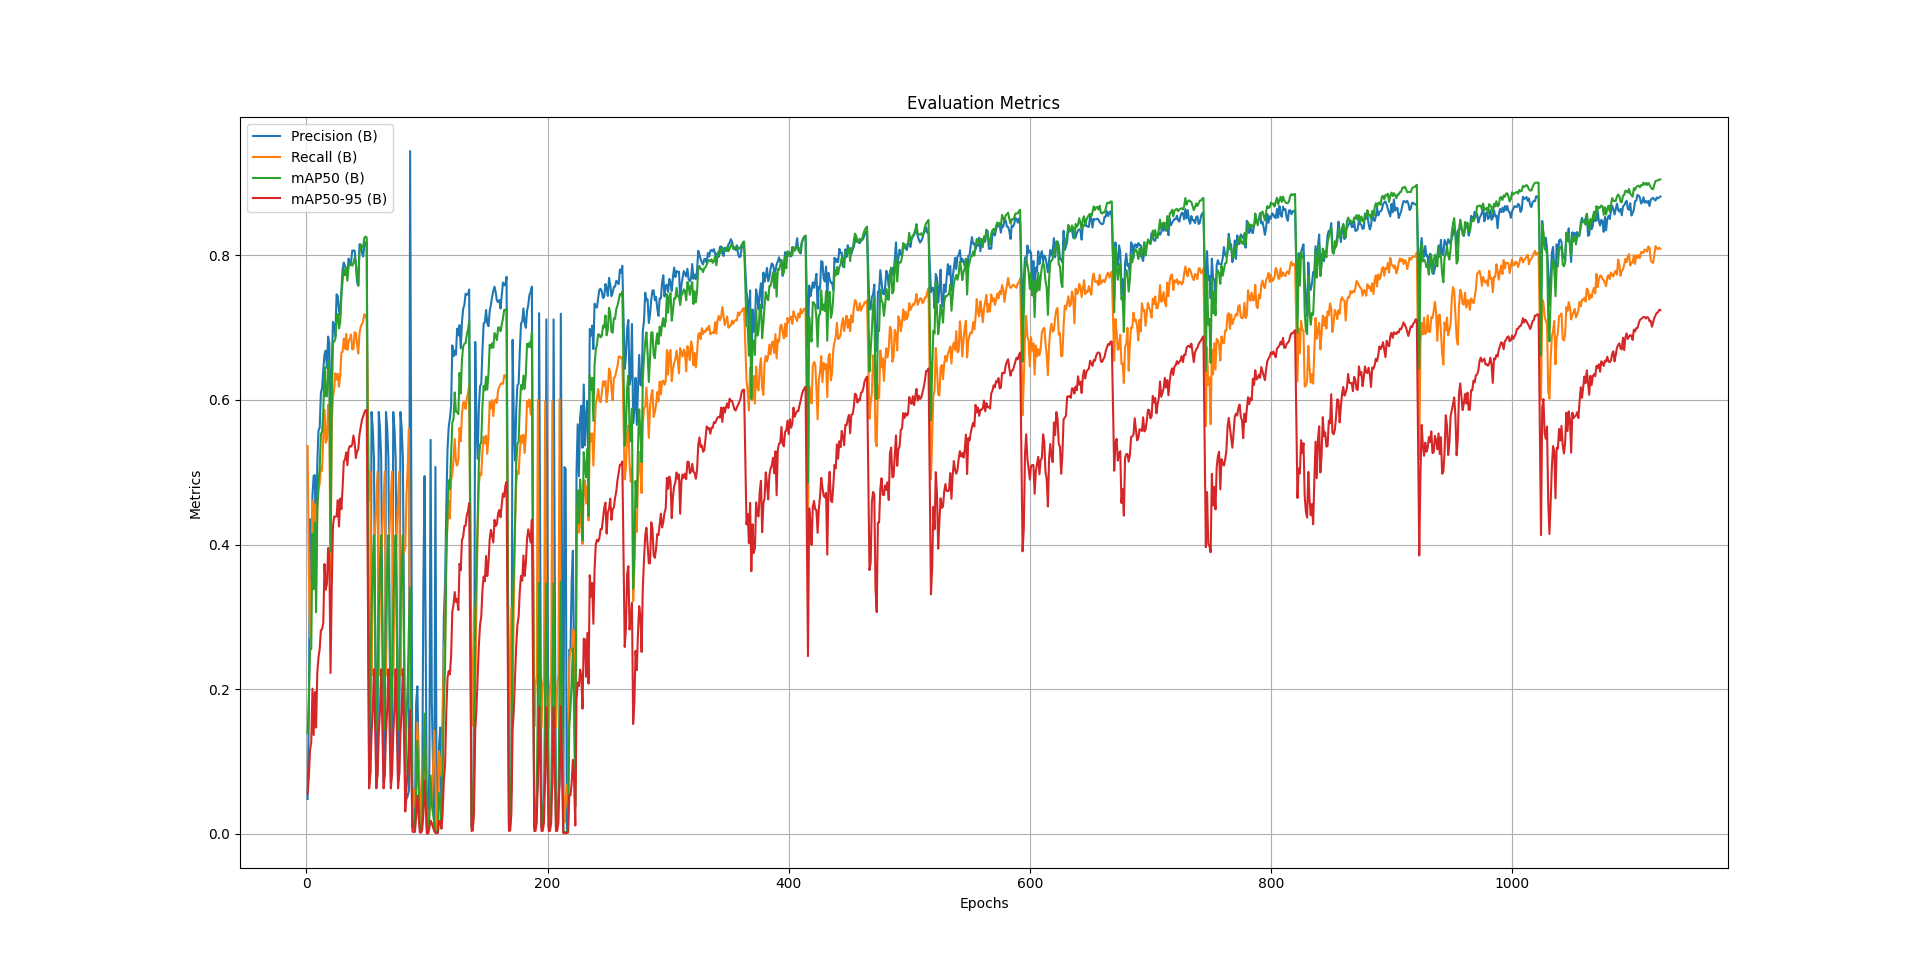
\includegraphics[scale=0.2]{Figure_3.png}
    \caption{
        The values of the four evaluation metrics 
        (Precision, Recall, mAP50, and mAP50-95) 
        improve steadily throughout the training process, 
        indicating that the model's performance enhances as training progresses. 
        The spikes in the plot reflect periods of fine-tuning and adjustments to the model’s weights.   
    }
    \label{fig:fig3}
\end{figure}

Figures 1, 
2, 
and 3 showcase the quantitative performance data of the machine learning model and provide valuable insights into its effectiveness and efficiency. 
By examining these plots, 
we can assess how the model's performance evolves over time, 
identify potential weaknesses or areas for improvement, 
and determine its ability to generalize to unseen data. 
Additionally, 
the plots reveal trends in the model's learning process, 
such as whether it is overfitting or underfitting. 
These quantitative metrics are essential for validating the model’s utility in real-world applications and guiding further refinement, 
ensuring that the model meets the desired standards for accuracy and reliability in tasks like parking space detection or any other specific objectives.


\subsection{Test Examples}

In Figure \ref{fig:fig4}, 
a test image from the dataset is presented with bounding boxes overlaid to indicate detected objects. 
Empty parking spaces are highlighted with green bounding boxes, 
while occupied spaces are marked with red. 
The YOLOv11 model successfully identifies and classifies parking spaces in this test image, 
demonstrating the model's ability to classify spaces in relative proximity.

However, 
as seen in Figure \ref{fig:fig5}, 
the model encounters challenges when objects are further away, 
particularly with identifying vehicles and parking spaces at a distance. 
This limitation arises from the model's struggle to accurately detect and classify objects farther from the camera, 
likely due to the reduced resolution of distant objects and the difficulty distinguishing fine details at greater distances. 
The frame shown in Figure \ref{fig:fig5} is from a test video, 
where this issue impacts the model’s performance.

The difficulty in detecting distant objects suggests that parking lots with large or irregular layouts will require multiple cameras to ensure complete coverage. 
By placing cameras strategically throughout the lot, 
it will be possible to mitigate the model's struggles with distant detections, 
ensuring that all parking spaces, 
both near and far, 
are adequately monitored and classified. 
This approach will improve the system's overall accuracy and ensure more reliable performance across a broader area.

\begin{figure}[h]
    \centering
    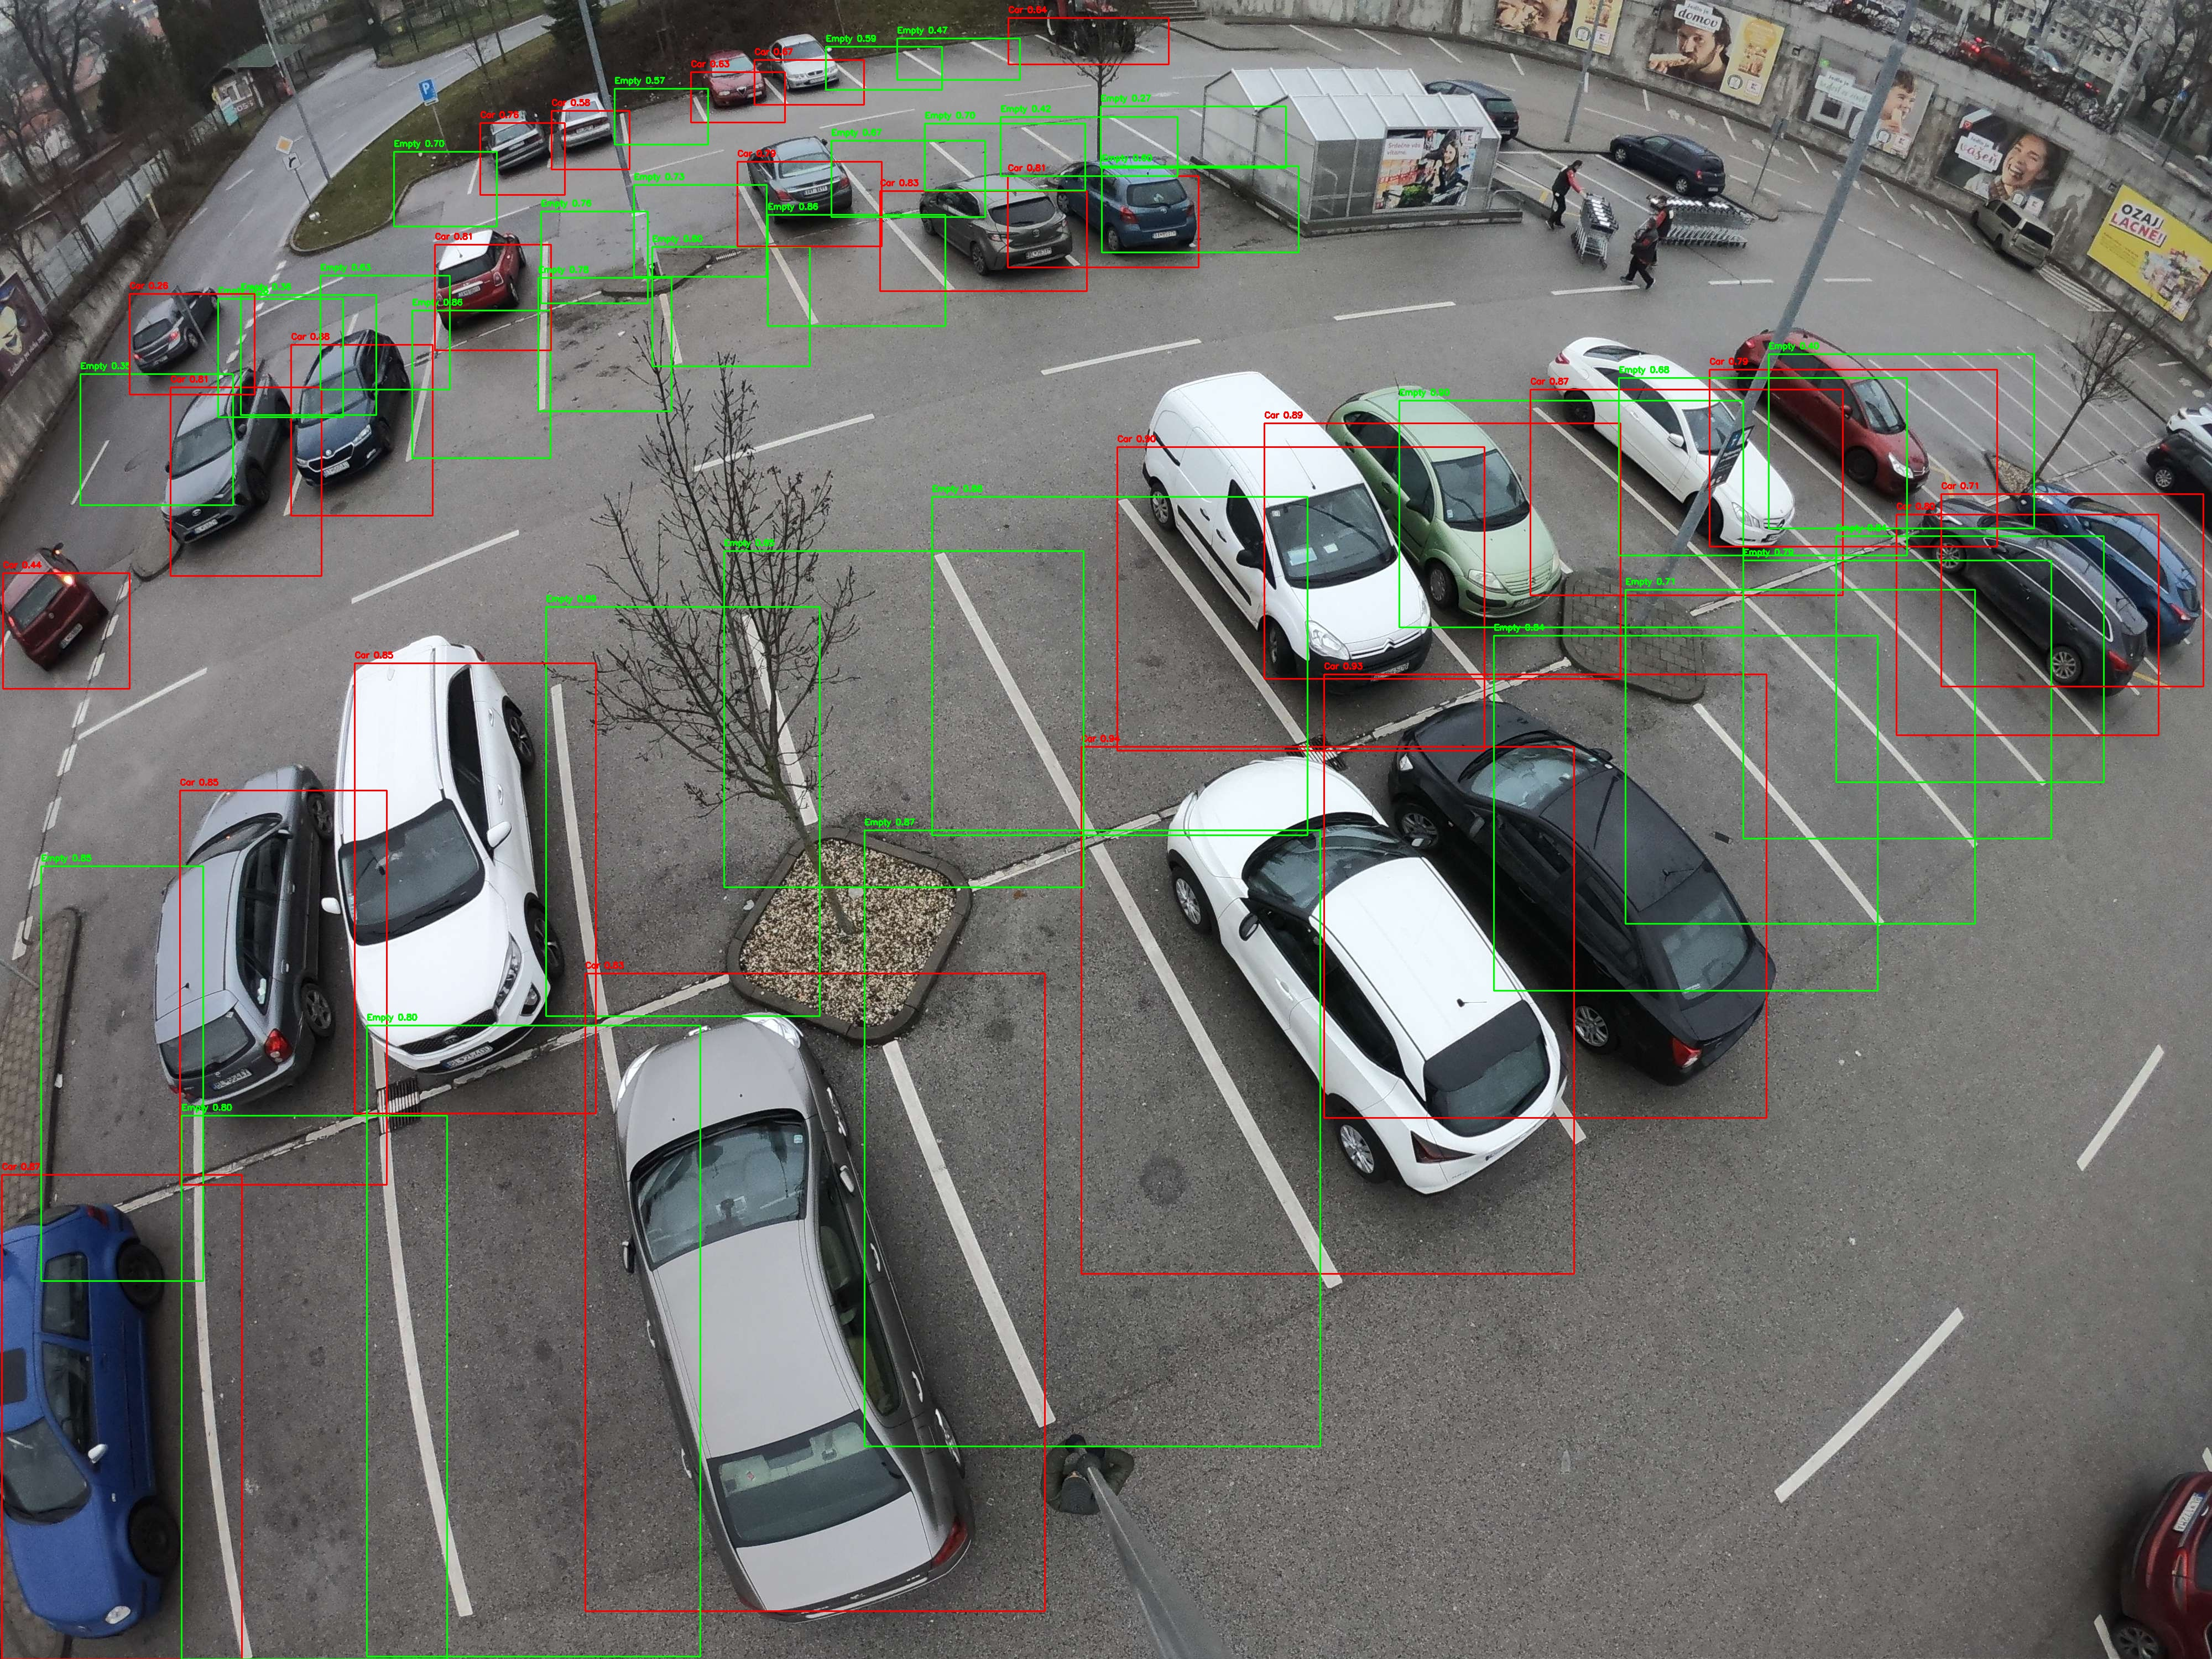
\includegraphics[scale=0.065]{Figure_4.JPG}
    \caption{
        Observe that the empty parking spaces are marked with green bounding boxes while occupied spaces are marked with red bounding boxes. 
        The YOLOv11 model correctly identifies and classifies spaces in the test data.
    }
    \label{fig:fig4}
\end{figure}

\begin{figure}[h]
    \centering
    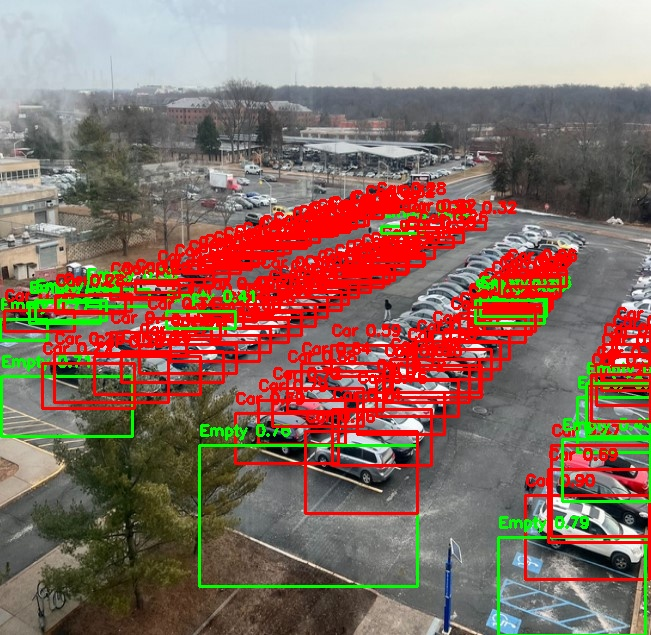
\includegraphics[scale=0.4]{Figure_5.JPG}
    \caption{
        Observe that the model struggles to identify vehicles and spaces at a distance. 
        Most lots will need more than one camera in order to cover every space. 
        This is a frame taken from a test video.   
    }
    \label{fig:fig5}
\end{figure}

Figures 4 and 5 are examples of qualitative data, 
which refers to non-numeric information that describes the characteristics or qualities of an object, 
phenomenon, 
or system. 
It can encompass user experiences or feedback regarding the ease of navigation within the parking lot, 
the availability of parking spaces during peak hours, 
or the overall safety and accessibility of the facility. 
Qualitative data is often subjective and focuses on the attributes or features that can't be easily quantified but provide essential insights for improving the user experience, 
operational efficiency, 
and service quality. 
Figure 5 provides a visual example of the model working and finding open and closed parking spaces.

\section{Cost/Sustainability analysis}

This project involves the development of a smart parking space detection system using a Raspberry Pi 5 (8GB) and a tilt-enabled camera setup. 
The system identifies empty and occupied parking spots to optimize parking efficiency and reduce time spent by drivers searching for available spaces. 
The prototype cost is approximately \$196.66, 
which includes the Raspberry Pi (\$80), 
tilt camera module (\$86.71), 
power supply (\$12), 
bumper (\$3), 
and a 64GB SD card (\$14.95). 
The estimated cost for mass production is approximately \$200 per unit, 
reflecting a cost-effective solution even at scale, 
especially considering the modularity and wide availability of its components.

Economically, 
the project is designed with affordability and scalability in mind. 
If deployed across large parking structures or citywide networks, 
further cost optimizations could be achieved through bulk procurement or centralized processing to reduce the need for one Raspberry Pi per camera. 
The system’s energy-efficient design also contributes to lower long-term operational costs, 
and potential tax incentives for smart city infrastructure, 
carbon footprint reduction, 
and energy-efficient technologies may reduce implementation expenses. 
Additionally, 
the system may provide indirect cost savings by lowering vehicle idling time, 
reducing fuel consumption, 
and minimizing emissions due to inefficient parking behaviors.

Environmentally, 
the system contributes positively by reducing greenhouse gas emissions associated with drivers circling to find parking. 
The hardware components, 
such as the Raspberry Pi, 
have a low power footprint and can operate efficiently with minimal energy consumption. 
Furthermore, 
the use of commonly available and recyclable materials supports a sustainable product lifecycle. 
As the system minimizes unnecessary vehicle movement, 
it indirectly reduces urban traffic congestion and resource overuse.

Socially, 
the impact of the project is notable in its ability to improve urban mobility, 
reduce driver frustration, 
and promote smarter city planning. 
By streamlining the parking process, 
it increases accessibility for all, 
including the elderly and those with disabilities, 
and reduces stress in high-traffic zones. 
While partial automation may reduce the need for manual lot attendants, 
it simultaneously opens avenues for new tech-related roles in installation, 
maintenance, 
and data analysis.
The project also enhances public safety by reducing the chances of illegal or hazardous parking and complies with evolving regulations around smart infrastructure and urban sustainability.

\section{Computer Vision/Society}

The widespread adoption of machine vision technologies has transformed the landscape of urban infrastructure, placing robotics at the heart of contemporary societal innovation. 
These vision-based systems are foundational to the development of smart cities, 
enabling a range of applications from traffic management and surveillance to public service automation. 
By offering real-time visual interpretation, 
machine vision equips autonomous systems with the capability to interact meaningfully with dynamic environments. 
This capability enhances the efficiency, 
sustainability, 
and safety of urban operations, 
creating more responsive and adaptive cities. 
The integration of these systems into daily infrastructure allows for continuous monitoring and intelligent decision-making, 
ultimately improving the quality of urban life.

Recent technological advances have made it possible to implement vision-based object detection and tracking using efficient and lightweight methods. 
For instance, 
techniques that utilize frame differencing, 
adaptive thresholding, 
and computationally simple tracking algorithms have been shown to detect moving objects in real time with minimal resource requirements, 
as discussed in \cite{wang_and_zhang}. 
These approaches are particularly valuable in settings where hardware limitations or cost constraints are a concern, 
offering affordable yet effective alternatives to more complex and hardware-intensive systems. 
In parallel, 
deep learning methods, 
particularly those based on convolutional neural networks, 
have greatly improved the accuracy and responsiveness of object detection systems. 
Models like YOLO exemplify this progress by achieving a balance between inference speed and detection accuracy, allowing real-time application in a range of real-world scenarios.

One domain where these technologies have had a pronounced impact is in urban mobility, 
especially through the deployment of smart parking systems. 
The study presented in \cite{smart_parking} 
illustrates how machine vision can be employed to identify and classify parking spaces, 
thereby reducing traffic congestion, 
lowering emissions from idling vehicles, 
and improving the overall efficiency of urban space utilization. 
By continuously monitoring parking availability and conveying that information to users, 
such systems streamline parking behavior, 
reduce driver frustration, 
and facilitate more informed urban planning. 
Automating this process also diminishes the reliance on human labor and surveillance, 
helping cities manage increasing transportation demands without incurring proportional operational costs. 
The ability to collect and analyze real-time data further allows city planners and policymakers to make data-driven decisions that enhance infrastructure planning and resource allocation.

However, 
the integration of machine vision into public spaces also introduces a range of ethical challenges, 
particularly related to privacy, 
consent, 
and data governance. 
Surveillance systems that rely on visual data may inadvertently capture sensitive or personally identifiable information, 
prompting concerns about individual rights and data protection. 
While traditional surveillance often depends on biometric recognition, 
modern machine vision systems, 
such as those employing YOLO-based detection, 
can be configured to focus solely on non-personal elements like objects or vehicles. 
This approach offers a partial solution to privacy issues, 
but it is not sufficient on its own. 
Ethical deployment of such systems requires a framework that incorporates privacy by design, 
transparency in data usage, 
and clear accountability for misuse or data breaches. 
Ensuring community trust and stakeholder involvement in the planning and implementation phases is essential for sustainable adoption.

The role of robotics in public service extends beyond transportation and surveillance into fields such as healthcare, 
education, 
and environmental monitoring. 
As \cite{social_robotics} discusses, 
the evolution of social robotics demonstrates how these systems can contribute meaningfully to human-centered services. 
In healthcare settings, 
vision-enabled robots can assist in patient monitoring, 
therapeutic interventions, 
and routine administrative tasks, 
easing the burden on medical professionals and improving patient outcomes. 
In educational environments, 
robotics systems equipped with perception capabilities can support personalized learning experiences, 
provide interactive content, 
and engage students in novel ways. 
These applications reflect a broader trend of using robotics not merely as tools of automation but as collaborative agents that address specific societal needs, especially in underserved communities.

Another critical area of advancement is the integration of computer vision with IoT in transportation systems, 
which has proven especially valuable in rapidly growing regions such as Southeast Asia. 
These areas often face acute challenges due to increasing urbanization, 
vehicle density, 
and inconsistent infrastructure quality. 
As detailed in \cite{real_time_transport}, 
a robust object detection framework using YOLOv4 can reliably identify various traffic-related entities such as bikes, 
cars, 
cows, 
dogs, 
and pedestrians, 
in both urban and rural settings. 
Enhancing this framework, 
an IoT-based alert system for pothole detection utilizes GPS data and cloud-based messaging to inform drivers of road hazards, 
a critical feature during monsoon seasons when visibility is often compromised. 
Together, 
these components form a cohesive and scalable solution for intelligent transportation management, 
offering tangible improvements in commuter safety and operational efficiency.

The increasing incorporation of robotic perception into civic systems reflects a significant transformation in how societies view technology. 
It marks a shift from seeing automation solely as a means of industrial efficiency to recognizing its role in supporting social infrastructure. 
This shift raises fundamental questions about the governance of these technologies, 
including who is responsible for their oversight, 
how inclusive their benefits are, 
and how equitably they are deployed. 
The continued success of robotics in urban infrastructure depends not only on technical advancements but also on how well these systems align with public values, 
ethical norms, 
and regulatory frameworks. 
Societal acceptance and the long-term sustainability of these technologies require transparent development practices, 
inclusive design, 
and community engagement.

In this evolving context, 
even comparatively low-cost systems such as YOLO-based parking detection provide critical insight into the opportunities and limitations of integrating robotics into public environments. 
These systems exemplify how intelligent technologies can be deployed effectively without requiring prohibitively expensive resources, 
making them accessible to a wider array of municipalities and institutions. 
By studying the deployment, 
functionality, 
and societal impact of such technologies, 
researchers and policymakers can derive valuable lessons that inform future applications. 
These include considerations around privacy, 
data integrity, 
user experience, 
and system resilience. 
Ultimately, 
the thoughtful integration of machine vision into public infrastructure holds the promise of not only enhancing operational efficiency but also fostering more equitable, 
inclusive, 
and responsive urban environments.



\section{Conclusion}

The project envisions a highly scalable and adaptable system capable of being deployed in a wide range of environments, 
including shopping malls, 
stadiums, 
airports, 
university campuses, 
and densely populated urban centers. 
Its modular design ensures seamless integration with existing infrastructure, 
making it suitable for both small-scale and large-scale parking facilities. 
By leveraging the portability and affordability of edge devices such as Raspberry Pi, 
the system remains cost-effective while maintaining reliable performance. 
This flexibility opens opportunities for widespread adoption, 
especially in developing regions or in contexts where large-scale infrastructure investments are not feasible.

Looking ahead, 
several enhancements are planned to increase the system's intelligence, 
responsiveness, 
and utility. 
These include integration with smart city frameworks to deliver real-time traffic and parking analytics, 
aiding not only drivers but also city planners and municipal authorities \cite{smart_cities}. 
Predictive modeling techniques using machine learning can be applied to forecast parking space availability based on historical usage patterns and live sensor inputs, 
optimizing traffic flow and minimizing time spent searching for parking. 
The architecture can also be extended into multi-camera or drone-assisted configurations, 
enabling coverage of vast and dynamic environments such as open-air lots or event venues. 
Drones on predetermined flight paths could provide aerial perspectives, 
increasing monitoring flexibility and responsiveness. 
By combining state-of-the-art machine vision with user-centric design principles, 
this system presents a forward-thinking, 
practical solution to the persistent challenges of urban parking, 
paving the way for smarter, more efficient cities.

The system can be further enhanced by integrating the Raspberry Pi with existing security camera infrastructures, 
offering a highly cost-effective and non-invasive solution for upgrading current parking management systems. 
This approach significantly reduces the need for expensive hardware installations and complex system overhauls, 
making it a practical choice for a wide range of environments. 
By connecting Raspberry Pi devices to cameras that are already in place, 
the system can seamlessly leverage the video streams from these cameras to monitor parking space occupancy in real-time \cite{parking_space_management}. 
This method not only ensures enhanced performance and affordability but also allows for easy scalability, 
as it can be quickly deployed in both small-scale parking lots and large, 
complex environments. 
By transforming existing security infrastructure into smart, 
responsive parking management systems, 
this solution maximizes the utility of current resources while providing a robust, 
efficient, 
and flexible tool for modern urban parking challenges.

\section{References}

\printbibliography

\newpage

\onecolumn

\section{Appendix - Code}

\inputminted{python}{inference_export.py}

\end{document}
